\documentclass[a4paper,oneside,10pt]{book}
\usepackage[utf8]{inputenc}
\usepackage{amsmath}
\usepackage{color}
\usepackage{graphicx}
\usepackage{colortbl}
\usepackage{amssymb}
\usepackage{amsthm}
\usepackage{accents}
\usepackage{mathtools}
\usepackage[T1]{fontenc}
\usepackage{placeins}
\usepackage{graphicx}
\usepackage{float}
\usepackage{multicol}
\usepackage{hyperref}
\title{Algorytm Faracha}
\author{Bartosz Wodziński}
\pagenumbering{gobble}
\newtheorem*{theorem}{Twierdzenie}

\begin{document}
\maketitle
    \section*{Cel algorytmu i format wejścia}
    Wejściem do algorytmu jest słowo $w$ o długości $n$ nad alfabetem $\Sigma = [n]$ - liczb naturalnych od $1$ do $n$. Zakładać będziemy, że $n = 2^k$ - jeśli nie, to można słowo $w$ wydłużyć o czynnik liniowy, tak żeby ta równość zachodziła, dodając na koniec odpowiednią ilość $'\$'$, a po wykonaniu algorytmu ``uciąć'' z drzewa sufiksowego poddrzewa odpowiadające tym symbolom. \\ \\
    Algorytm tworzy drzewo sufiksowe dla tego słowa w czasie $O(n)$. Od drzewa wymagane jest, aby dla każdego wierzchołka, krawędzie prowadzące do jego dzieci posortowane były leksykograficznie względem ich etykiet (w przypadku liczb naturalnych porządek leksykograficzny rozumiemy jako zdefiniowany przez zwykłą relację $<$).
    
    \section*{Idea algorytmu}
    Algorytm Faracha działa rekurencyjnie i każdy jego etap można zapisać w trzech krokach:
    \begin{enumerate}
     \item Zbuduj drzewo sufiksowe $T_o$ dla \textit{nieparzystych} sufiksów, czyli takich, które zaczynają się od nieparzystego indeksu (numerujemy od $1$).
     \item Korzystając z drzewa $T_o$, zbuduj drzewo $T_e$ - drzewo sufiksowe dla \textit{parzystych} sufiksów (bez wywołania rekurencyjnego!).
     \item Połącz drzewa $T_o$ i $T_e$ w jedno drzewo $T$.
    \end{enumerate}
    Jeśli kroki $2.$ i $3$ będziemy w stanie wykonać w liniowej złożoności, to wówczas cały algorytm będzie miał złożoność:
    $$
        T(n) = T\left(\frac{n}{2}\right) + O(n),
    $$
    a więc liniową. \\
    Aby  uniknąć dodatkowego wywołania rekurencyjnego w równaniu (co zwiększyłoby złożoność do $O(nlgn)$), drzewo $T_e$ konstruowane będzie bezpośrednio z drzewa $T_o$.
    
    \section*{Tworzenie drzewa $T_o$}
    Tworzenie drzewa nieparzystych sufiksów przebiega w kilku krokach:
    \begin{enumerate}
     \item $\forall i \in [\frac{n}{2}]$ stwórz parę $\langle w[2i-1], w[2i] \rangle$ i wszystkie takie pary umieść w liście $S'$ i każdą z nich zamień na jej \textit{rangę} (indeks w posortowanej leksykograficznie liście). Na przykład, dla słowa \verb|121112212221|, lista $S'$ wygląda tak: \\
     \verb|[(1,2), (1,1), (1,2), (2,1), (2,2), (2,1), #]|, a po zamianie elementów na ich rangi, tak: \\
     \verb|[2,1,2,3,4,3,#]|.
     \item Rekurencyjnie oblicz $T_{S'}$ - drzewo sufiksowe dla słowa $S'$ oraz jego tablicę sufiksową składającą się z $A_{T_{S'}}$ - posortowanej tablicy sufiksów i z $LCP_{T_{S'}}$ - tablicy najdłuższych wspólnych prefiksów dla $A_{T_{S'}}$.
     \item Korzystając z $A_{T_{S'}}$, oblicz $A_{T_o}$ w następujący sposób:
     $$
        A_{T_o}[i] = 2A_{T_{S'}}[i] - 1,
     $$
     co bazuje na obserwacji, że każdy nieparzysty sufiks $w[2i-1]...w[n]$ jest równoważny sufiksowi $S'[i]...S'[\frac{n}{2}]$ (co wynika z konstrukcji $S'$), a zatem leksykograficzny porządek $A_{T_{S'}}$ jest taki sam jak porządek $A_{T_o}$. Jedyne co trzeba zmienić, to indeksy, odwracając przekształcenie z punktu $1.$: $\langle w[2i-1],w[2i] \rangle \rightarrow S'[i]$.
     \item Oblicz $LCP_{A_{T_o}}$, korzystając z $LCP_{A_{T_{S'}}}$, według wzoru:
      \begin{align*}
      \left.
       LCP_{T_o}[i] = 2LCP_{T_{S'}}[i] + \bigg\{
       \begin{array}{@{}l}
        1 \text{ if } w[A_{T_o}[i] + 2LCP_{T_{S'}}] = w[A_{T_o}[i+1] + 2LCP_{T_{S'}}[i]]   \\
        0 \text{ otherwise}
       \end{array},
        \right.              
      \end{align*}
      co również wynika z konstrukcji słowa $S'$.
    \item Na podstawie $A_{T_O}$ i $LCP_{T_o}$ skonstruuj drzewo $T_o$.
    \end{enumerate}
    \section*{Tworzenie drzewa $T_e$}
    \begin{enumerate}
     \item Wstępnie przetwórz drzewo $T_o$ (w czasie liniowym od jego rozmiaru) tak aby dało się odpowiadać na zapytania o \verb|lca| na tym drzewie w czasie stałym.
     \item Korzystając z obserwacji, że każdy parzysty sufiks to nieparzysty sufiks poprzedzony jednym znakiem, stwórz $A_{T_e}$. W tym kroku możemy wykorzystać obliczoną już listę $A_{T_o}$, ``dokleić'' odpowiedni znak przed każdym elementem $A_{T_o}$ i użyć sortowania pozycyjnego tylko dla tego pierwszego znaku.
     \item Oblicz tablicę $LCP_{T_e}$ korzystając z zapytań o \verb|lcp(word(a),word(b))|, czyli zapytań o \verb|lca(a,b)| w drzewie sufiksowym:
      \begin{align*}
      \left.
       lcp(w[2i,n],w[2j,n]) = \bigg\{
       \begin{array}{@{}l}
        lcp(w[2i+1,n],w[2j+1,n]) + 1 \text{ if } w[2i] = w[2j]   \\
        0 \text{ otherwise}
       \end{array},
        \right.              
      \end{align*}
      
      \item Stwórz $T_e$ w oparciu o $A_{T_e}$ i $LCP_{T_e}$.
    \end{enumerate}
    
\section*{Łączenie drzew $T_o$ i $T_e$}
Zauważmy, że aby stworzyć drzewo $T$ z drzew $T_o$ i $T_e$, wystarczy zbudować tablice $A_T$ i $LCP_T$. Do uzyskania tych tablic potrzebujemy móc szybko (w czasie stałym) odpowiadać na pytania o najdłuższy wspólny prefiks dwóch sąsiadujących sufiksów w tablicy $A_T$. Umożliwiającą nam to wyrocznię uzyskamy poprzez \textit{zachłanne} połączenie drzew $T_o$ i $T_e$. \\ \\
\textit{Zachłanne} połączenie $T'$ rozumiemy jako takie połączenie dwóch drzew ($T_e$ i $T_o$), w którym:
\begin{itemize}
 \item Każdy wierzchołek z tych drzew ma odpowiadający sobie wierzchołek w drzewie $T'$, a ponadto, jeśli $e \in T_e$, $o \in T_o$ i \verb|word(e) = word(o)|, to wierzchołkom $e$ i $o$ odpowiada ten sam wierzchołek $t \in T$. \\
 Wierzchołek $u$ \textit{odpowiada} wierzchołkowi $v \in T_o \vee v \in T_e$ wtedy i tylko wtedy gdy $|word(u)| = |word(v)|$, a ponadto dla każdego wierzchołka $a$ z $T_o$ (lub $T_e$), który jest na drodze z korzenia do wierzchołka $v$ zachodzi: $word(v)[|word(a)| + 1] = word(u)[|word(a)| + 1]$, czyli $word(v)$ i $word(u)$ są tej samej długości i zgadzają się przynajmniej na indeksach, które odpowiadają pierwszym znakom na każdej krawędzi na drodze z korzenia do $v$.
 \item Z każdego wierzchołka $t \in T$, dla dowolnych dwóch etykiet $w$, $v$ krawędzi z niego wychodzących zachodzi: $w[0] \ne v[0]$ ($w[1] \ne v[1]$ przy numeracji od $1$).
 \item Drzewo $T'$ nie zawiera żadnych innych wierzchołków.
\end{itemize}
W skrócie można powiedzieć, że $T'$ to drzewo, które powstaje dokładnie w ten sposób co naiwnie wykonane poprawne połączenie $T_o$ i $T_e$ do $T$, z tą tylko różnicą, że zamiast porónywać wszystkie znaki na odpowiednich krawędziach (powiedzmy $u$ i $v$) (i ewentualnie dzielić je jeśli różnią się na jakiejś pozycji), porównujemy tylko pierwsze znaki, a podział robimy tylko w miejscu, w którym skończy się krótsza z nich. Procedurę tworzenia $T'$ (czyli ``nałożenia na siebie'' drzew $T_o$ i $T_e$ patrząc tylko na pierwszy znak krawędzi) przedstawia poniższy rysunek:
\begin{center}
 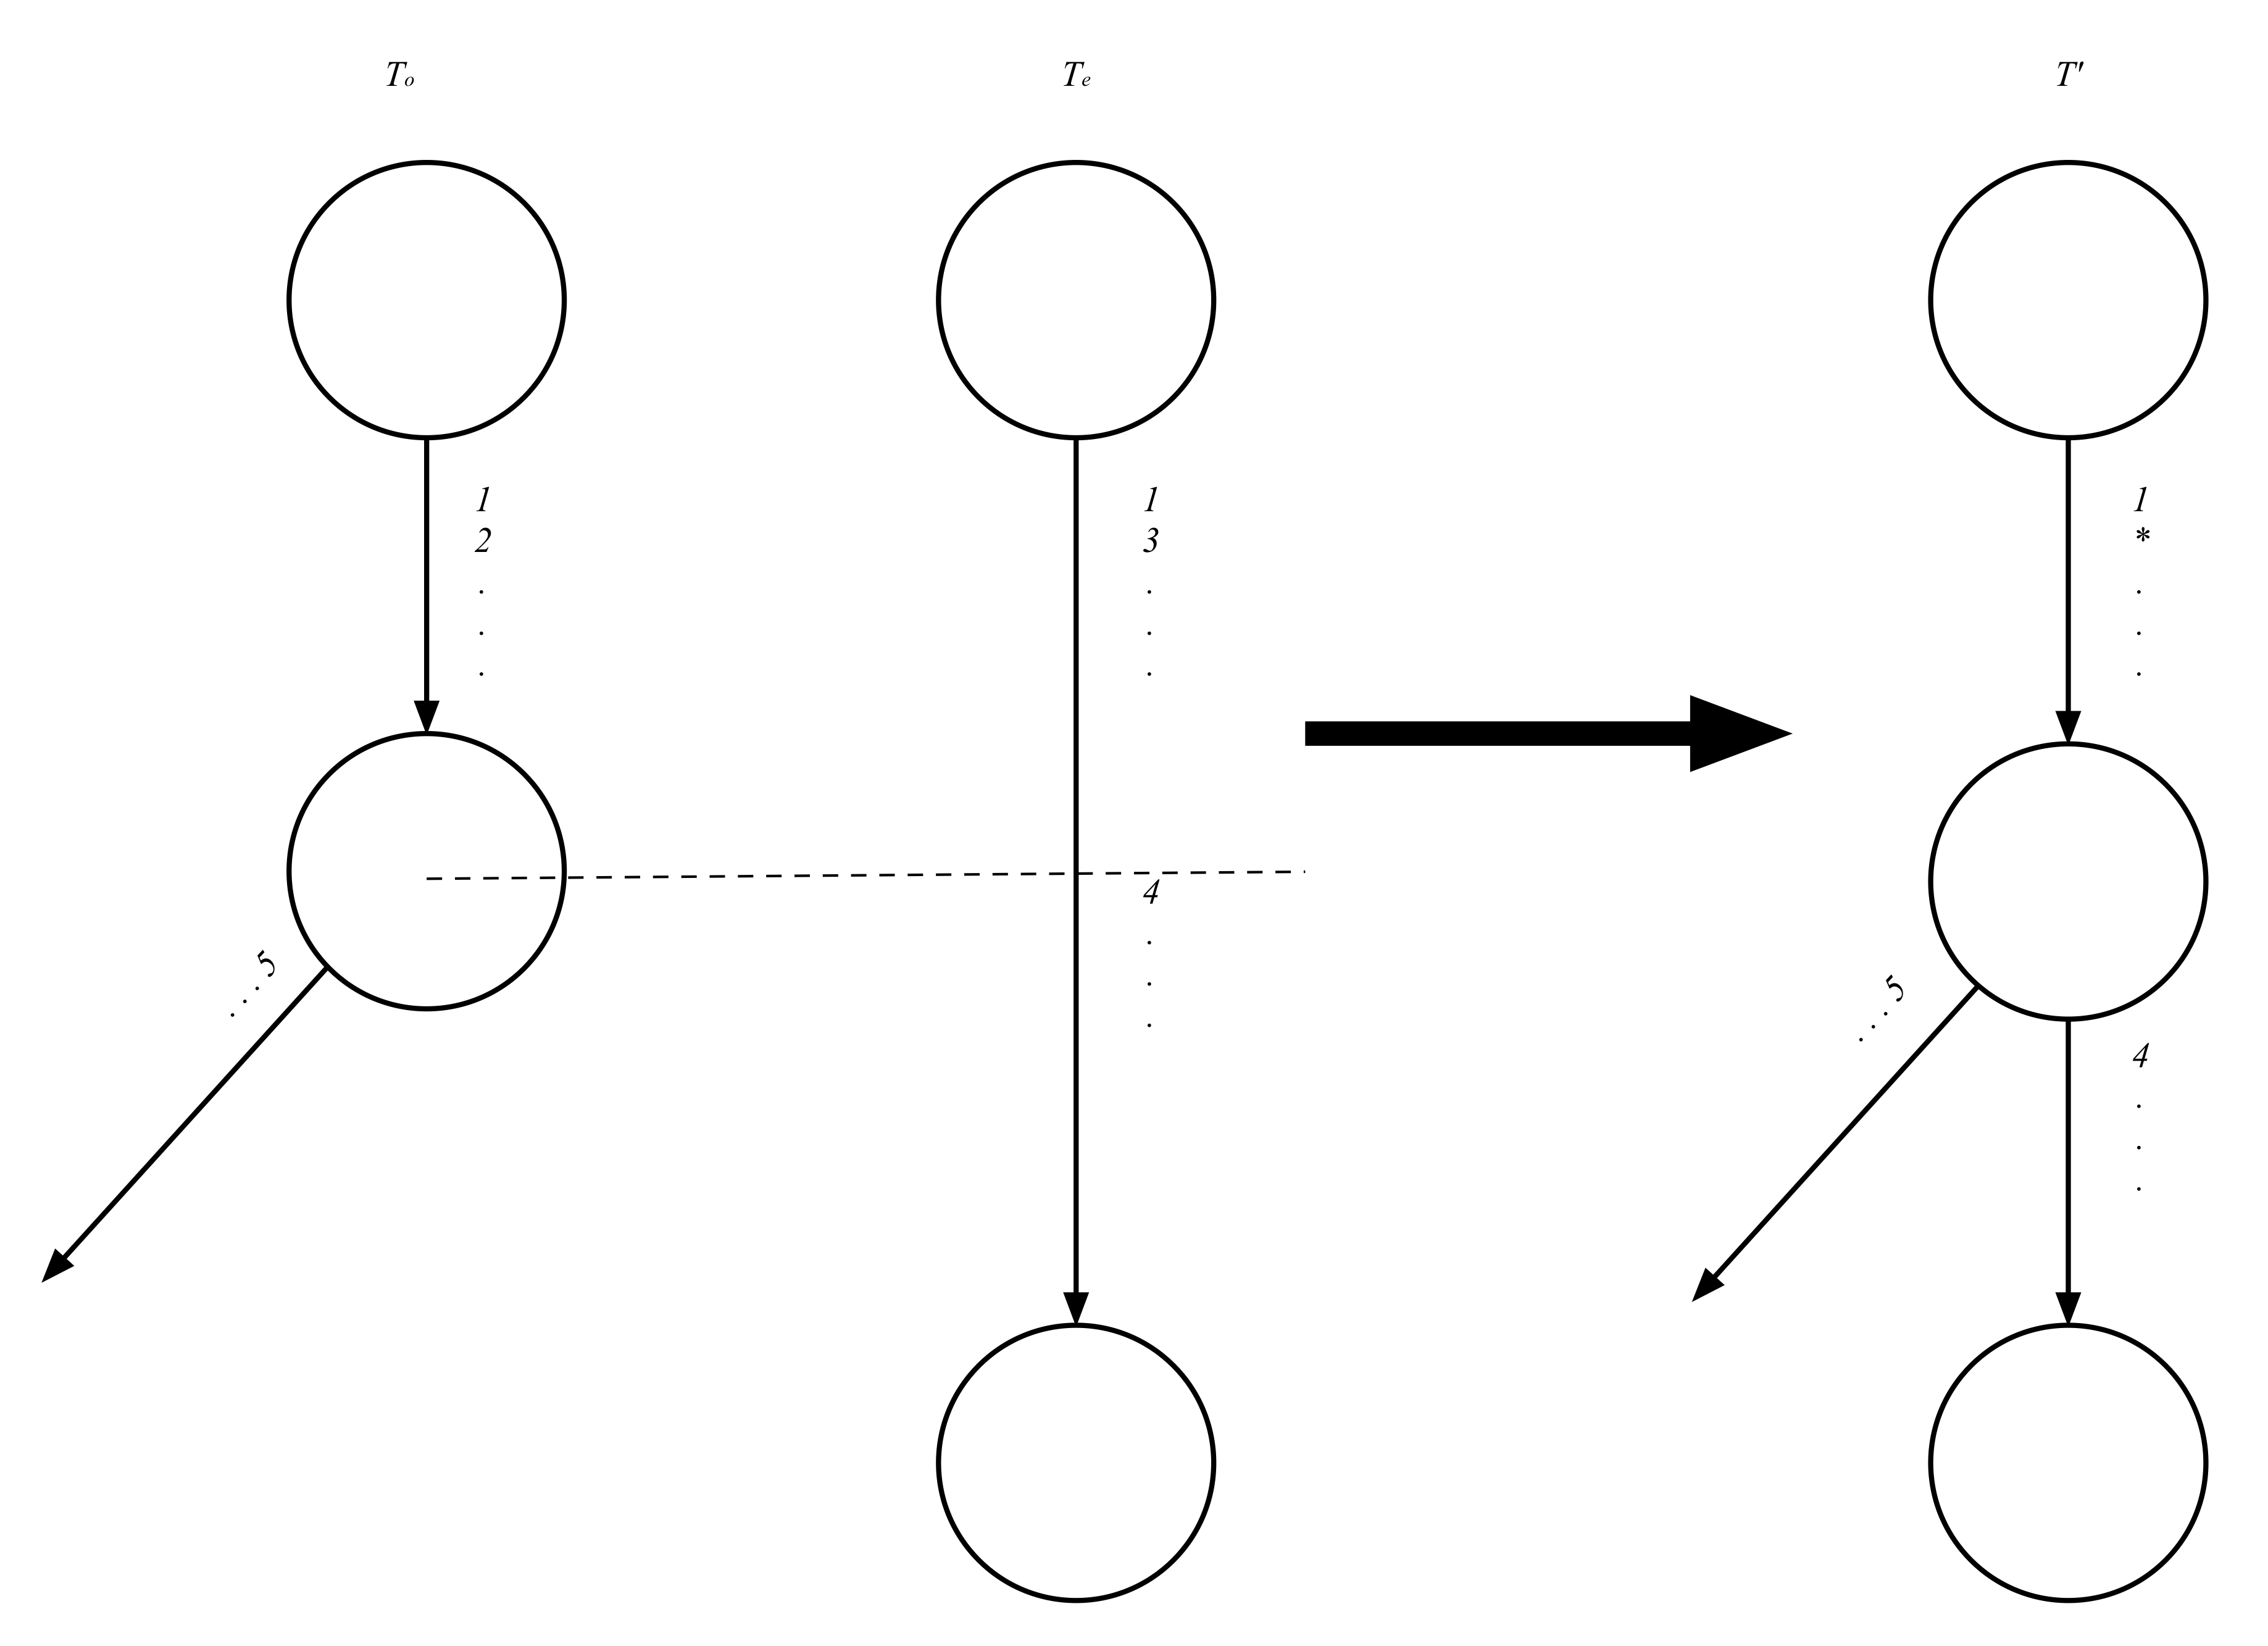
\includegraphics[scale=0.1,keepaspectratio=true]{../graphics/overmergingSuffixTrees.jpg}
 % overmergingSuffixTrees.jpg: 3674x2666 px, 72dpi, 129.61x94.05 cm, bb=0 0 3674 2666
\end{center}


Wiedząc jak jest konstruowane drzewo $T'$, zapiszmy kroki do stworzenia poprawnego drzewa $T$:
\begin{enumerate}
 \item Stwórz $T'$ tak jak zostało to wyżej opisane.
 \item Wierzchołek drzewa $T'$, który ma odpowiadający wierzchołek w $T_o$ nazwijmy \textit{nieparzystym}, a jeśli ma odpowiadający wierzchołek w $T_e$, to nazwijmy go \textit{parzystym}. Pewne wierzchołki (np. korzeń) mogą być zarówno parzyste jak i nieparzyste.\\
 Teraz, dla każdego wierzchołka $u \in T'$ znajdź parę wierzchołków (jeśli istnieje) $(a,b)$, które są jego potomkami i liśćmi drzewa, a ponadto $a$ jest parzysty, $b$ jest nieparzysty oraz \verb|lca(a,b) = u|. Załóżmy, że \\ \verb|word(a) = w[2i,n], word(b) = w[2j-1,n]|. Dodatkowo, każdemu liściowi $c$ takiemu, że \verb|word(c) = w[k,n]| nadajmy etykietę $l_k$. Zgodnie z tą konwencją $a = l_{2i}, \, b = l_{2j - 1}$.
 \\
 Zdefiniujmy funkcję $d$ taką, że $d(u) = lca(l_{2i+1}, l_{2j})$ i policzmy ją dla każdego $u$. Zauważmy, że jeśli $T'$ byłoby poprawnym drzewem, to $d(u) = suffix
\_link(u)$.
 \item Zakładając, że funkcja $d$ definiuje drzewo, dla każdego wierzchołka $u$ policz jego głębokość $L(u)$ w tym drzewie. Skorzystaj z faktu, że $lcp(w[2i,n], w[2j-1]) = L(lca(l_{2i}, l_{2j-1}))$ i stwórz tablicę $LCP_T$. 
\end{enumerate}
\section*{Dowód poprawności}
Wystarczy udowodnić poprawność punktów $2.$ i $3.$
\begin{theorem}
Najdłuższy wspólny prefiks dowolnej pary liści $(a,b)$, takich, że $a$ - parzysty, $b$ - nieparzysty, i takich, że \verb|lca|$(a,b) = u$, jest taki sam.
\end{theorem}
\begin{proof}[Dowód]
Weźmy wierzchołek parzysty $u$ mający zarówno parzystego jak i nieparzystego potomka. Weźmy teraz dwóch parzystych potomków (być może takich samych) $u$: $l_{2i},\,l_{2j}$. Wówczas, \verb|lcp|$(w[2i,n],w[2j,n]) \geq |word(u)|$, ponieważ $u$, $l_{2i}$, $l_{2j}$ były w drzewie $T_e$.


Teraz, weźmy parę $l_{2i'-1}$, $l_{2j'-1}$ potomków $u$. Zachodzi wtedy \verb|lcp|$(w[2i'-1,n],w[2j'-1,n]) \geq |word(u)|$. Jest tak, ponieważ, jeśli $u$ był również w $T_o$, to działa ten sam argument co poprzednio. Jeśli nie był w $T_o$, to ponieważ $l_{2i'-1}$, $l_{2j'-1}$ są liśćmi, to musi istnieć wierzchołek $u' = $\verb| lca|$(l_{2i'-1}, l_{2j'-1}) \in T_o$, który jest potomkiem $u$ w $T'$. 


Rozważmy teraz parę liści $l_{2i''}$ i $l_{2j''-1}$ w $T'$, takich że $u = $\verb| lca|$(l_{2i''}, l_{2j''-1})$. Zachodzi wtedy \verb|lcp|$(w[2i'',n], w[2j''-1, n]) \leq |word(u)|$. Wynika to z faktu, że jeśli byłoby inaczej, to wtedy więcej niż jedna krawędź wychodząca z $u$ zaczynała by się tym samym znakiem, co jednak w $T'$ nie ma miejsca. Analogiczne rozumowanie możemy przeprowaddzić dla $u$ będącego wierzchołkiem nieparzystym i wówczas każda z powyższych nierówności również będzie zachodziła.

Weźmy w końcu liście $l_{2i'},$, $l_{2i''}$, $l_{2j'-1}$, $l_{2j''-1}$ takie, że \verb|lca|$(l_{2i'}, l_{2j'-1}) = $ \verb| lca|$(l_{2i''}, l_{2j''-1}) = u$. Wtedy, \verb|lcp|$(w[2i',n], w[2j'-1,n]) = k \leq |word(u)|$, co udowodniliśmy przed chwilą. Wiemy jednak, że \verb|lcp|$(w[2i',n], w[2i'',n]) \geq |word(u)| \geq k$, a zatem musi być \verb|lcp|$(w[2i'',n], w[2j'-1,n]) = k$. Podobnie, \verb|lcp|$(w[2i'',n], w[2j''-1,n]) = k$. Wobec tego: \\
\verb|lcp|$(w[2i',n],w[2j'-1,n]) = $\verb| lcp|$(w[2i'',n], w[2j''-1,n]) = k$.
\end{proof}

\begin{theorem}
Funkcja $d$ definiuje drzewo na wierzchołkach $T'$, a ponadto dla dowolnych $l_{2i}$ i $l_{2j-1}$ zachodzi $L($\verb|lca|$(l_{2i}, l_{2j-1})) = $\verb| lcp|$(w[2i,n], w[2j-1,n])$.
\end{theorem}
\begin{proof}[Dowód]
Dowód jest indukcyjny ze względu na długość \verb|lcp|. Jeśli \verb|lcp|$word[2i, n], word[2j-1,n]) = 0$, to wówczas $word[2i, n]$ i $word[2j-1,n]$ różnią się na pierwszym znaku, więc \verb|lca|$(l_{2i}, l_{2j-1}) = $\verb| root|, co wynika ze sposobu konstruowania drzewa $T'$.

Załóżmy teraz, że twierdzenie zachodzi dla pary sufiksów parzystych i nieparzystych, takich, że ich \verb|lcp| $< k$. Niech $l_{2i},\,l_{2j-1}$ będą liśćmi takimi, że \verb|lca|$(w[2i,n], w[2j-1,n]) = k > 0$. Ponadto, niech $u = $\verb| lca|$(l_{2i}, l_{2j-1})$. Wtedy $u$ nie jest korzeniem, bo $k > 0$.

Niech teraz $l_{2i'}$, $l_{2j'-1}$ będą liśćmi użytymi do zdefiniowania $d(u)$. Zatem, z definicji, $d(u) = $\verb| lca|$(l_{2i'+1},l_{2j'})$.

Z założeń indukcyjnych wiemy, że funkcja $d$ definiuje drzewo na dotychczas rozważonych wierzchołkach, a ponadto, że funkcja $L$ jest zdefiniowana na tych wierzchołkach i że zwraca poprawne wartości \verb|lcp|. Zatem, z faktu, że funkcja $d$ definiuje drzewo, wiemy że $L(u) = 1 + L(d(u))$. Ponadto, z faktu, że funkcja $L$ zwraca poprawne wartości dla dotychczas rozważonych wierzchołków wiemy, że $1 + L(d(u)) = 1 + $\verb| lcp|$(w[2i'+1,n],w[2j',n])$. Teraz, ponieważ $k > 0$ (w szczególności oznacza to, że $w[2i'] = w[2j'-1]$), zachodzi $1 + $\verb| lcp|$(w[2i'+1,n],w[2j',n]) = $\verb| lcp|$(w[2i',n],w[2j'-1,n])$. A z poprzedniego twierdzenia wiemy, że \verb|lcp|$(w[2i',n],w[2j'-1,n]) = $\verb| lcp|$(w[2i,n],w[2j-1,n])$.

Wobec tego, $L(u) = $\verb| lcp|$(w[2i,n],w[2j-1,n])$, a ponadto struktura zdefiniowana przez funkcję $d$ jest drzewem.
\end{proof}

\section*{Złożoność}
\subsection*{Tworzenie $T_o$}
\begin{enumerate}
\item Sortowanie pozycyjne dla par, w których maksymalna liczba jest mniejsza lub równa $n$ (tak jest, bo początkowe słowo spełnia to założenie, a każde następne powstaje przez zastąpienie elementu przez jego rangę) zajmuje $O(n)$ czasu.
\item Jeśli wszystkie inne kroki będą liniowe, to ten krok zajmie $T(n) = T(\frac{n}{2}) + O(n) = O(n)$ czasu.
\item Każdy element tablicy $A_{T_o}$ liczymy w czasie stałym, więc ten krok zajmuje $O(n)$ czasu.
\item Podobnie jak w poprzednim punkcie, mamy stały czas na przetworzenie jednego elementu tablicy, więc całość robimy w $O(n)$.
\item Jest możliwe skonstruowanie drzewa sufiksowego w czasie liniowym z tablic $A$ i $LCP$.\\ Idea: wstawiamy kolejne sufiksy w kolejności leksykograficznej. Po wstawieniu każdego sufiksu, zatrzymujemy się w liściu, który go reprezentuje i dopóki \verb|lcp|$(word(v), next\_suffix) < |word(v)|$ wykonujemy, $v = v.parent$, a następnie dodajemy nową krawędź z wierzchołka $v$ albo dzielimy już wychodzącą.
\end{enumerate}
\subsection*{Tworzenie $T_e$}
\begin{enumerate}
\item Da się w czasie liniowym zrobić preprocessing drzewa tak aby w czasie stałym odpowiadać na zapytania \verb|lca|. Jest to nietrywialny algorytm, który jest opisany w \url{https://www.ics.uci.edu/~eppstein/261/BenFar-LCA-00.pdf}.
\item Sortowanie pozycyjne na liczbach nieprzekraczających $n$ działą w $O(n)$.
\item Ponieważ zapytania o \verb|lcp| przetwarzane są w czasie stałym, czas działania tego kroku to $O(n)$.
\item Analogicznie jak dla $T_o$ - $O(n)$.
\end{enumerate}
\subsection*{Łączenie drzew $T_o$ i $T_e$}
\begin{enumerate}
\item Ten krok to zwykły DFS działający liniowo względem sumarycznej ilości wierzchołków w drzewach $T_o$ i $T_e$, a ponieważ są to poprawne drzewa sufiksowe, to mają liniowe rozmiary względem $O(\frac{n}{2})$.
\item Odpowiednią parę liści dla każdego wierzchołka z $T'$ możemy znaleźć przy pomocy jednego DFS-a, korzystając z obliczonych wcześniej wartości dla potomków tego wierzchołka.

Funkcję $d$ liczymy dla każdego wierzchołka w czasie stałym, po wcześniejszym liniowym przetworzeniu drzewa $T'$ do zapytań o \verb|lca|.
\item Głębokość w drzewie liczymy ponownie używając algorytmu DFS i korzystając z obliczonych wartości, każdy element $LCP_T$ liczymy w czasie stałym. Odtworzenie drzewa z tablic $A_T$ i $LCP_T$ wykonujemy w czasie $O(n)$, jak wyżej.
\end{enumerate}
\end{document}
